\documentclass[10pt]{article}
\usepackage[a4paper,margin=1.5cm]{geometry}
\usepackage[T1]{fontenc}
\usepackage{tgpagella,mathpazo}
\usepackage[scaled=.95]{helvet}
\usepackage[dvipsnames]{xcolor}
\usepackage{graphicx,tikz,booktabs,tabularx}
\usetikzlibrary{arrows.meta,positioning,calc,backgrounds}
% Shared manuscript and TikZ visual language for the OPERA paper.
% Keep colours and Helvetica-like figure typography synchronized with
% opera/visualization/style.py (Arial/Liberation Sans on render hosts).

\definecolor{OperaIndigo}{HTML}{2D3A8C}
\definecolor{OperaNavy}{HTML}{1A237E}
\definecolor{OperaPeriwinkle}{HTML}{5C7AEA}
\definecolor{OperaSlate}{HTML}{737D8C}
\definecolor{OperaTeal}{HTML}{408579}
\definecolor{OperaGreen}{HTML}{1B7A4A}
\definecolor{OperaSienna}{HTML}{B5451B}
\definecolor{OperaTerracotta}{HTML}{C16A58}
\definecolor{OperaOchre}{HTML}{B18B4D}
\definecolor{OperaLavender}{HTML}{8974AC}
\definecolor{OperaInk}{HTML}{17212B}
\definecolor{OperaInkSecondary}{HTML}{485463}
\definecolor{OperaInkMuted}{HTML}{657180}
\definecolor{OperaBorder}{HTML}{CBD2DA}
\definecolor{OperaGrid}{HTML}{E8ECF1}
\definecolor{OperaPaper}{HTML}{F7F8FA}

\tikzset{
  opera/.style={font=\sffamily\small, text=OperaInk},
  panel/.style={draw=none, fill=white, inner sep=0pt},
  softpanel/.style={
    rounded corners=0.8mm,
    draw=OperaGrid,
    line width=0.45pt,
    fill=OperaPaper,
    inner sep=2.4mm,
  },
  stage/.style={
    rounded corners=0.7mm,
    draw=OperaBorder,
    line width=0.6pt,
    fill=white,
    align=center,
    minimum height=8mm,
    inner xsep=3mm,
    inner ysep=1.8mm,
  },
  stageblue/.style={stage, draw=OperaIndigo!55, fill=OperaIndigo!7},
  stageteal/.style={stage, draw=OperaTeal!65, fill=OperaTeal!8},
  stagewarm/.style={stage, draw=OperaSienna!60, fill=OperaSienna!7},
  latent/.style={
    circle,
    draw=OperaIndigo!65,
    fill=OperaIndigo!9,
    line width=0.6pt,
    minimum size=6mm,
    inner sep=0pt,
    font=\sffamily\scriptsize\bfseries,
  },
  token/.style={
    rounded corners=0.7mm,
    draw=OperaBorder,
    fill=white,
    minimum width=6.2mm,
    minimum height=4.8mm,
    inner sep=0.5mm,
    font=\sffamily\tiny,
    align=center,
  },
  outcome/.style={
    rounded corners=1mm,
    draw=OperaTerracotta!70,
    fill=OperaTerracotta!9,
    minimum height=5.8mm,
    inner xsep=1.8mm,
    font=\sffamily\scriptsize,
    align=center,
  },
  flow/.style={
    -{Latex[length=2mm,width=1.2mm]},
    line width=0.75pt,
    draw=OperaInkSecondary,
  },
  flowblue/.style={flow, draw=OperaIndigo},
  flowteal/.style={flow, draw=OperaTeal},
  flowwarm/.style={flow, draw=OperaSienna},
  relation/.style={
    -{Latex[length=1.8mm,width=1.1mm]},
    line width=0.65pt,
    draw=OperaLavender,
    densely dashed,
  },
  captionnote/.style={
    font=\sffamily\fontsize{6.6}{7.5}\selectfont,
    text=OperaInkMuted,
    align=center,
  },
  labelsmall/.style={
    font=\sffamily\fontsize{7}{8}\selectfont,
    text=OperaInkSecondary,
    align=center,
  },
  heading/.style={
    font=\sffamily\fontsize{9}{10}\selectfont\bfseries,
    text=OperaInk,
    align=left,
  },
  panelletter/.style={font=\sffamily\bfseries\normalsize, text=OperaInk},
  divider/.style={draw=OperaBorder, line width=0.45pt},
  eyebrow/.style={font=\sffamily\fontsize{6.5}{7.5}\selectfont\bfseries,
    text=OperaIndigo, align=left},
}

\pagestyle{empty}
\begin{document}
\section*{The disease--outcome grid as the study's visual language}
\resizebox{\textwidth}{!}{% Supervision scopes drawn as four copies of the Fig. 2B disease-outcome matrix:
% same axes, rows/columns, ellipses, cell geometry, lavender gradient, sienna
% target and teal borrowing spokes. Filled cells are supervised tasks; pale
% outlined cells are present in the panel but not supervised by that fit.
% Lines are illustrative sharing paths, not learned gates or measured routes.
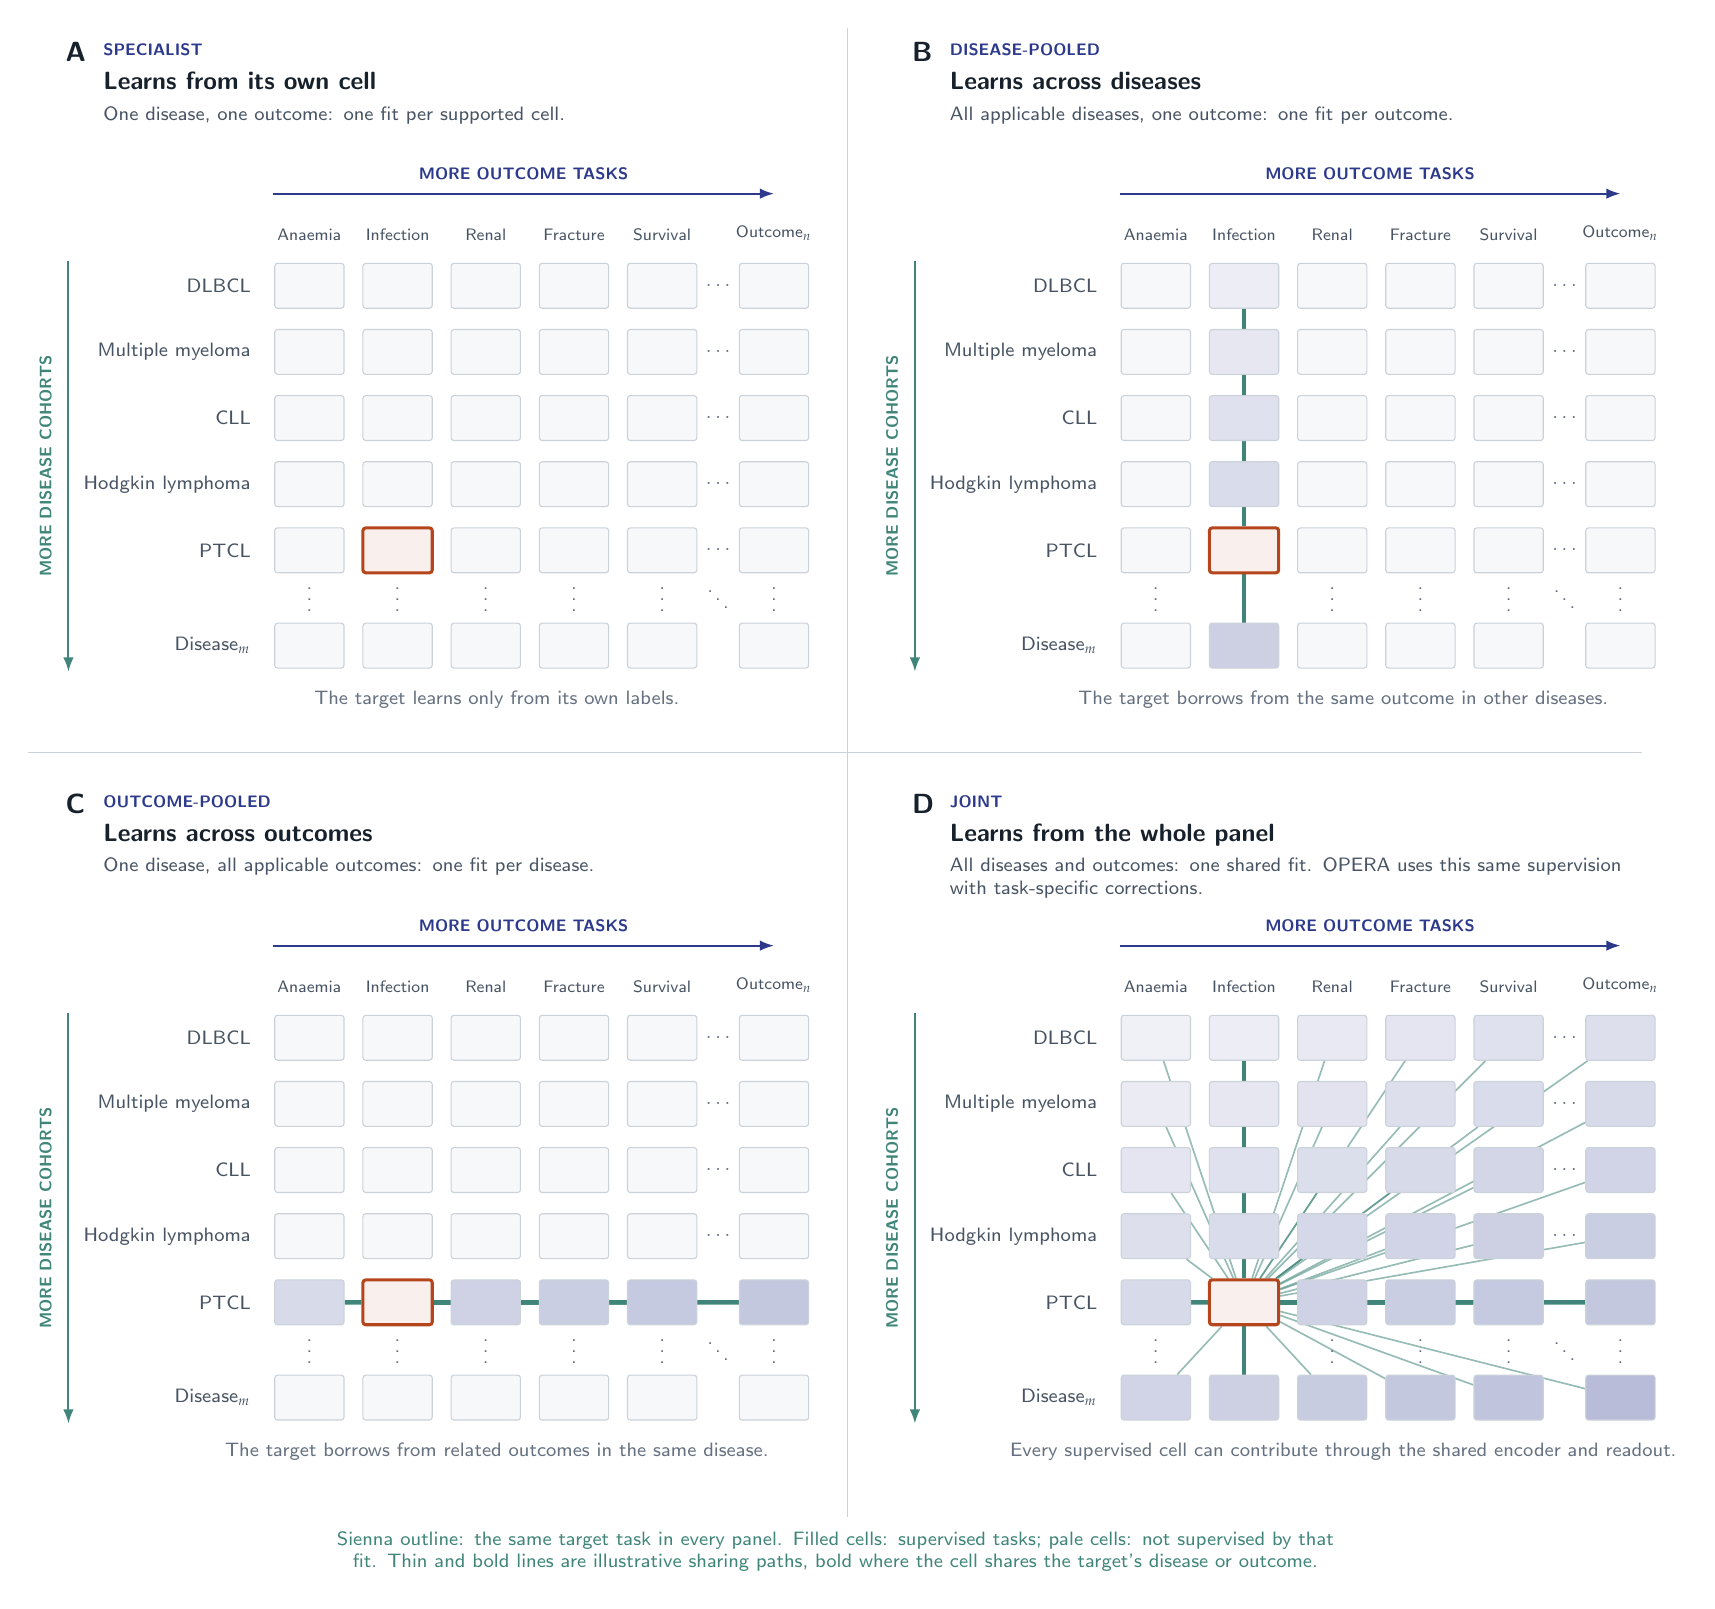
\begin{tikzpicture}[opera,x=1cm,y=1cm]
\foreach \scopeid/\sx/\sy/\letter/\eyebrowtext/\title/\sub/\note in {
 S/0/0/A/{SPECIALIST}/{Learns from its own cell}/{One disease, one outcome: one fit per supported cell.}/{The target learns only from its own labels.},
 D/10.75/0/B/{DISEASE-POOLED}/{Learns across diseases}/{All applicable diseases, one outcome: one fit per outcome.}/{The target borrows from the same outcome in other diseases.},
 O/0/-9.55/C/{OUTCOME-POOLED}/{Learns across outcomes}/{One disease, all applicable outcomes: one fit per disease.}/{The target borrows from related outcomes in the same disease.},
 J/10.75/-9.55/D/{JOINT}/{Learns from the whole panel}/{All diseases and outcomes: one shared fit. OPERA uses this same supervision with task-specific corrections.}/{Every supervised cell can contribute through the shared encoder and readout.}}{
\begin{scope}[xshift=\sx cm,yshift=\sy cm]
 \node[panelletter,anchor=north west] at (0,0) {\letter};
 \node[eyebrow,anchor=north west] at (.48,-.03) {\eyebrowtext};
 \node[heading,anchor=north west] at (.48,-.38) {\title};
 \node[labelsmall,anchor=north west,align=left,text width=8.6cm] at (.48,-.82) {\sub};
 \begin{scope}[yshift=-5mm]
 % Axes exactly as in Fig. 2B.
 \draw[-{Latex[length=1.8mm]},draw=OperaIndigo,line width=.75pt] (2.76,-1.55)--(9.12,-1.55);
 \node[eyebrow,text=OperaIndigo] at (5.94,-1.30) {MORE OUTCOME TASKS};
 \foreach \r/\disease in {0/DLBCL,1/Multiple myeloma,2/CLL,3/Hodgkin lymphoma,4/PTCL}
  \node[labelsmall,anchor=east] at (2.60,-2.72-.84*\r) {\disease};
 \draw[-{Latex[length=1.8mm]},draw=OperaTeal,line width=.75pt] (.16,-2.40)--(.16,-7.62);
 \node[eyebrow,text=OperaTeal,rotate=90] at (-.13,-5.01) {MORE DISEASE COHORTS};
 \foreach \col/\outcome in {0/Anaemia,1/Infection,2/Renal,3/Fracture,4/Survival}
  \node[font=\sffamily\fontsize{6.2}{7}\selectfont,text=OperaInkSecondary,
   align=center,text width=1.05cm,anchor=south] at (3.22+1.12*\col,-2.27) {\outcome};
 \node[font=\sffamily\fontsize{6.2}{7}\selectfont,text=OperaInkSecondary,
  align=center,text width=1.05cm,anchor=south] at (9.12,-2.27) {Outcome$_n$};
 % Main 5 x 5 block. Supervision depends on the scope; the target is row 4, column 1.
 \foreach \r in {0,...,4}{\foreach \col in {0,...,4}{
  \def\active{0}
  \if\scopeid D \ifnum\col=1 \def\active{1}\fi\fi
  \if\scopeid O \ifnum\r=4 \def\active{1}\fi\fi
  \if\scopeid J \def\active{1}\fi
  \def\tone{OperaPaper}
  \ifnum\active=1 \pgfmathtruncatemacro{\shade}{7+3*\r+2*\col}\edef\tone{OperaIndigo!\shade}\fi
  \node[rounded corners=.35mm,draw=OperaBorder,fill=\tone,
   minimum width=8.8mm,minimum height=5.7mm] (\scopeid m\r\col) at (3.22+1.12*\col,-2.72-.84*\r) {};
 }}
 \foreach \r in {0,...,4}{
  \node[font=\sffamily\scriptsize,text=OperaInkMuted] at (8.41,-2.72-.84*\r) {$\cdots$};
  \def\active{0}
  \if\scopeid O \ifnum\r=4 \def\active{1}\fi\fi
  \if\scopeid J \def\active{1}\fi
  \def\tone{OperaPaper}
  \ifnum\active=1 \pgfmathtruncatemacro{\shade}{16+3*\r}\edef\tone{OperaIndigo!\shade}\fi
  \node[rounded corners=.35mm,draw=OperaBorder,fill=\tone,
   minimum width=8.8mm,minimum height=5.7mm] (\scopeid n\r) at (9.12,-2.72-.84*\r) {};
 }
 \foreach \x in {3.22,4.34,5.46,6.58,7.70,9.12}{
  \node[font=\sffamily\scriptsize,text=OperaInkMuted] at (\x,-6.60) {$\vdots$};
 }
 \node[font=\sffamily\scriptsize,text=OperaInkMuted] at (8.41,-6.60) {$\ddots$};
 \node[labelsmall,anchor=east] at (2.60,-7.29) {Disease$_m$};
 \foreach \col in {0,...,4}{
  \def\active{0}
  \if\scopeid D \ifnum\col=1 \def\active{1}\fi\fi
  \if\scopeid J \def\active{1}\fi
  \def\tone{OperaPaper}
  \ifnum\active=1 \pgfmathtruncatemacro{\shade}{22+2*\col}\edef\tone{OperaIndigo!\shade}\fi
  \node[rounded corners=.35mm,draw=OperaBorder,fill=\tone,
   minimum width=8.8mm,minimum height=5.7mm] (\scopeid z\col) at (3.22+1.12*\col,-7.29) {};
 }
 \def\tone{OperaPaper}
 \if\scopeid J \def\tone{OperaIndigo!34}\fi
 \node[rounded corners=.35mm,draw=OperaBorder,fill=\tone,
  minimum width=8.8mm,minimum height=5.7mm] (\scopeid zn) at (9.12,-7.29) {};
 \node[rounded corners=.35mm,draw=OperaSienna,line width=1.1pt,fill=OperaSienna!8,
  minimum width=8.8mm,minimum height=5.7mm] (\scopeid target) at (4.34,-6.08) {};
 % Spokes from supervised cells only: bold when the cell shares the target's
 % outcome (column 1) or disease (row 4), thin otherwise, as in Fig. 2B.
 \begin{scope}[on background layer]
  \foreach \r in {0,...,4}{\foreach \col in {0,...,4}{
   \def\link{0}
   \if\scopeid D \ifnum\col=1 \def\link{1}\fi\fi
   \if\scopeid O \ifnum\r=4 \def\link{1}\fi\fi
   \if\scopeid J \def\link{1}\fi
   \ifnum\r=4 \ifnum\col=1 \def\link{0}\fi\fi
   \ifnum\link=1
    \def\bold{0}
    \ifnum\col=1 \def\bold{1}\fi
    \ifnum\r=4 \def\bold{1}\fi
    \ifnum\bold=1
     \draw[draw=OperaTeal,opacity=1,line width=1.6pt] (\scopeid m\r\col)--(\scopeid target);
    \else
     \draw[draw=OperaTeal,opacity=.55,line width=.6pt] (\scopeid m\r\col)--(\scopeid target);
    \fi
   \fi
  }}
  \if\scopeid O \draw[draw=OperaTeal,opacity=1,line width=1.6pt] (\scopeid n4)--(\scopeid target);\fi
  \if\scopeid D \draw[draw=OperaTeal,opacity=1,line width=1.6pt] (\scopeid z1)--(\scopeid target);\fi
  \if\scopeid J
   \foreach \r in {0,...,3}{\draw[draw=OperaTeal,opacity=.55,line width=.6pt] (\scopeid n\r)--(\scopeid target);}
   \draw[draw=OperaTeal,opacity=1,line width=1.6pt] (\scopeid n4)--(\scopeid target);
   \foreach \col in {0,2,3,4}{\draw[draw=OperaTeal,opacity=.55,line width=.6pt] (\scopeid z\col)--(\scopeid target);}
   \draw[draw=OperaTeal,opacity=1,line width=1.6pt] (\scopeid z1)--(\scopeid target);
   \draw[draw=OperaTeal,opacity=.55,line width=.6pt] (\scopeid zn)--(\scopeid target);
  \fi
 \end{scope}
 \node[captionnote,text width=8.5cm] at (5.60,-7.98) {\note};
 \end{scope}
\end{scope}
}
\draw[divider] (10.05,.05)--(10.05,-18.85);
\draw[divider] (-.35,-9.15)--(20.15,-9.15);
\node[labelsmall,text=OperaTeal,align=center,text width=18cm] at (9.90,-19.30)
 {Sienna outline: the same target task in every panel. Filled cells: supervised tasks; pale cells: not supervised by that fit.
 Thin and bold lines are illustrative sharing paths, bold where the cell shares the target's disease or outcome.};
\end{tikzpicture}
}

\vspace{5mm}
\noindent\textbf{The two experiments must look different.}
Filled cells show supervised training scope. Small badges or a second layer
show the readout (shared BCE or selected router). Encoder-origin labels sit
above the same grid: local, external-direct, external plus local DAPT.
Changing a source bank must not erase training cells.

\section*{Figure outline}
\begin{tabularx}{\textwidth}{@{}lXX@{}}
\toprule
Display & Grid-inspired layout & Scientific question \\
\midrule
Figure 1 & S/D/O/J panels, common target outline, temporal split underneath & What supervision does each model receive? \\
Figure 2 & Disease--outcome effect maps for D--S and O--S; adjacent J--O/J--D contrasts and rarity curves & Which pooling axis helps, and where? \\
Figure 3 & Shared, specialist, router and XGBoost absolute/paired results on aligned target rows & Does sharing improve on strong tabular prediction? \\
Figure 4 & Three encoder columns (local, external, external+DAPT), two readout rows (shared, router) & What do external pretraining and adaptation add? \\
Supplement & Full six-horizon atlas, source-bank factorial, calibration, patient/era strata, coverage, compute & How stable, interpretable and broadly supported are the findings? \\
\bottomrule
\end{tabularx}

\vspace{5mm}
\noindent\textbf{Conventions.} Diseases remain rows and outcomes remain columns
in every figure. The target cell is outlined in sienna; fills encode training
availability or empirical effect only when the legend says which. In results
maps, use a zero-centered diverging scale and mask unsupported cells explicitly.
Each metric has its own scale. Routing arrows are directional and weighted;
they are not observed patient outcomes or proof of beneficial transfer.
This outline contains no empirical performance values.
\end{document}
